\section{模型的建立与求解}

\subsection{问题1-1:结合解析几何,建立被动接受信号无人机的定位模型}

针对于问题(1),需要建立坐标系确定各无人机的位置,并引入相关数学模型使各无人机涉及到的参量具有数学关系,进一步加强对定位模型合理准确的建立。分析题目可知,可以用的坐标系有极坐标和空间直角坐标。对极坐标而言,当题目已确定无人机群处于同一个高度平面,所以可以引入极径$\rho$与极角$\alpha$两个因变量。对于空间直角坐标而言,至少存在两个以上的因变量,依题意对于无人机群控制在同一高度则可令$z=\alpha$,其中$x$与$y$为确定单无人机的具体位置。本文建立了基于同高度且按圆周均匀分布的间接式立体定位模型,通过对单无人机逐个编队,使之形成均匀圆周分布的定位模型。

\begin{figure}[h]
    \centering
    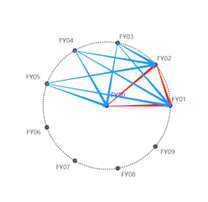
\includegraphics{res/AerialView.png}
    \caption{空间立体鸟瞰图}
\end{figure}

\textbf{模型一的建立——空间立体直角坐标定位模型}

依题意在空间直角坐标系中 是确定的,假定引入一参照物观测站(相对于原点 ),定位模型处于空间直角坐标系中,则无人机所到目标位置的真实坐标为 ,无人机观测站的坐标为 。各无人机到目标之间的距离为
 (1-1)

令

\begin{equation}
\begin{cases}
    r^2 = x_t^2 + y_t^2 + z_t^2   \\
    r^2_i = x_i^2 + y_i^2 + z_i^2 \\
\end{cases}
\label{e5-081538}
\end{equation}

在\eqref{e5-081537}式中,$r$为目标位置与坐标原点之间的距离,对\eqref{e5-081537}式平方联立\eqref{e5-081538}式可以得到\cite{weilian*feileGailulunjiqiyingyong}

\begin{equation}
\rho^2_i - r^2_i - r
= -2(x_ix_t + y_iy_t + z_iz_t)
\label{e5-081539}
\end{equation}

既有:

\begin{equation}
    \begin{cases}
        \rho_1^2 - r_1^2 - r^2 = -2(x_1x_t + y_1y_t + z_1z_t)   \\
        \rho_2^2 - r_2^2 - r^2 = -2(x_2x_t + y_2y_t + z_2z_t)   \\
        \rho_3^2 - r_3^2 - r^2 = -2(x_3x_t + y_3y_t + z_3z_5)   \\ 
    \end{cases}
\end{equation}

既有传统定位方程如\eqref{e5-081539}式所示,将其写成为矩阵形式有:

\begin{equation}
    A_1x_t = B_1
\end{equation}

其中:

\begin{equation}
    B_1=
    \left[
    \begin{matrix}
        \rho_1^2 - r_1^2 - r^2 \\
        \rho_2^2 - r_2^2 - r^2 \\
        \rho_3^2 - r_3^2 - r^2 \\
    \end{matrix}
    \right]
    A_1=
    \left[
    \begin{matrix}
        -2x_1 - 2y_1 - 2z_1 \\
        -2x_2 - 2y_2 - 2z_2 \\
        -2x_3 - 2y_3 - 2z_3 \\
    \end{matrix}
    \right]
    \notag
\end{equation}

计算上式,目标大致为$x_0$为:

\begin{equation}
    x_0 = A_1^{-1}B_1
    \label{e5-081704}
\end{equation}

引入偏差$\varepsilon_{\rho i}$构建定位方程为:

\begin{equation}
    \rho_i = \|x_i - x_t\| + \varepsilon_{\rho i}, i=1,2,3
\end{equation}

令$\varepsilon_{\rho i}~N(0, \sigma_\rho^2)$,将上式右边于$x_0$处进行泰勒展开并忽略最高项得到:

\begin{equation}
    \rho_i = \|x_i-x_0\|
    - \frac{(x_i-x_0)(x_t-x_0)}{\|x_i-x_0\|}
    - \frac{(y_i-y_0)(y_t-y_0)}{\|x_i-x_0\|}
    - \frac{(z_i-z_0)(z_t-z_0)}{\|x_i-x_0\|}
    + \varepsilon_{\rho i}
\end{equation}

得到初步定位方程,写成矩阵形式如下:

\begin{equation}
    Ay=B
    \label{e5-matrix}
\end{equation}

在\eqref{e5-matrix}式中:

\begin{equation}
    A=
    \left[
    \begin{matrix}
        \frac{x_1-x_0}{\rho'_1} & \frac{y_1-y_0}{\rho'_1} & \frac{z_1-z_0}{\rho'_1} \\

        \frac{x_2-x_0}{\rho'_2} & \frac{y_2-y_0}{\rho'_2} & \frac{z_2-z_0}{\rho'_2} \\
        
        \frac{x_3-x_0}{\rho'_3} & \frac{y_3-y_0}{\rho'_3} & \frac{z_3-z_0}{\rho'_3} \\
    \end{matrix}
    \right]
    y=
    \left[
        \begin{matrix}
            x_t - x_0   \\
            y_t - y_0   \\
            z_t - z_0   \\
        \end{matrix}
    \right]
\end{equation}

且

\begin{equation}
    B=
    \left[
        \begin{matrix}
            \rho'_1-\rho_1+\varepsilon_{\rho1} \\
            \rho'_2-\rho_2+\varepsilon_{\rho2} \\
            \rho'_3-\rho_3+\varepsilon_{\rho3} \\
        \end{matrix}
    \right]
    \|x_i - x_0\| = \rho'_i
\end{equation}

综上可解得初步定位方程得解为:

\begin{equation}
    y=A^{-1}B
\end{equation}

令无人机观测站站址偏差为$\Delta x_i$,且满足$\Delta x_i~N(0,\sigma_i^2)$,引入方程\eqref{e5-081704}进而得到最终得定位方程为:

\begin{equation}
\left[
    \begin{matrix}
        \frac{x_i-x_0}{\rho'_i} - a_i\Delta x_i     &   \frac{y_i-y_0}{\rho'_i} - b_i\Delta x_i     &   \frac{z_i-z_0}{\rho'_i} - c_i\Delta x_i \\
    \end{matrix}
\right]
\left[
    \begin{matrix}
        x_t - x_0   \\
        y_t - y_0   \\
        z_t - z_0   \\
    \end{matrix}
\right]
=
\rho'_i - d\Delta x_i - \rho_i + \varepsilon_{\rho i}
\end{equation}

……

综上联立上式得表达式定位解为:

\begin{equation}
    y_{Tu}=
    \left (
        A^TH_y^{-2}A
        +
        \left (
            \frac{1}{2}\min\frac{E{c_{2i^2}}}{c_{li}^2\mu_i} +
            \frac{1}{2}\max\frac{E{c_{2i}^2}}{c_{li}^2\mu_i}
        \right )
    \right )
\end{equation}

\textbf{模型特征值检验}:为验证所提定位模型得有效性及适应性,本题对题设的假设条件进行带入检验,依题意即得$\alpha=40$,半径为常数$\rho$,既有$x=\rho\cos\alpha, y=\rho\sin\alpha,z=\theta$,$\theta$为常数。对假设检验数据有下:

\begin{table}[htp!]
    \centering
    \caption{空间坐标}
    \begin{tabular}{cccc}
        \hline
        编号&   坐标变换(极→直)&   编号&   坐标变换(极→直)  \\
        \hline

        0&  (0, 0)→(0, 0, 0)&  5& (10, 160)→(-9.4, 3.42, 0)   \\
        1&  (10, 0)→(10, 0, 0)&    6&  (10, 200)→(-9.4, -3.42, 0)    \\
        2& (10, 40)→(7.66, 6.43, 0)&    7&  (10, 240)→(-5, -8,66, 0)    \\
        3& (10, 80)→(1.74, 9.85, 0)&   8&  (10, 280)→(1.74, -9.85, 0)  \\
        4&  (10, 120)→(-5, 8.66, 0)&    9&  (10, 320)→(7.66, -6.43, 0)  \\

        \hline
    \end{tabular}
\end{table}

\textbf{Step 1:}插入符合题设数据
对符合第一小问的题设加入假定数据进行数据预处理,分别对编号00~09的十架无人机插入已知假定的空间坐标;

\textbf{Step2:}对空间坐标可用极坐标调节简化
对极坐标设置两个参数进行极坐标转换,即极坐标依据空间坐标而成三角函数的数学关系进行变换,设置理想的定位模型以便两坐标的参照对比;\cite{wangnengbinShujukuxitongjiaocheng}


\textbf{Step3:}导入相应数据进行模型检验。


\subsection{问题1-2:求解实现有效定位的无人机数量}

\subsubsection{模型的分析}

为了方便后文描述,在此引入三圆定位模型的概念。

\newtheorem{mythm}{定理}[section]
\begin{mythm}
    % \label{线段半径定理}
    在平面内,一线段两端(线段长度已知)和该线段垂直平分线上的一点所构成的角与该线段可构成圆及所得圆的半径。(本题以特殊角证明,但结论适用)
\end{mythm}

\begin{proof}
    设线段两端的端点为$a$和$b$,在线段$ab$垂直平分线上的点为$c$,连接线段$ac$和线段$bc$,分别做垂直平分线,相交于一点,此时可得一圆。设线段$ab$的长度为$l$,$\angle acb$的度数为$\alpha$。故有三角函数方程:

    \begin{equation}
        \frac{l}{\sin 2\alpha}=
        \frac{r}{\sin(\frac{\pi}{2}-\alpha)}
    \end{equation}

    解得

    \begin{equation}
        r=\frac{l}{2\sin\alpha}
    \end{equation}
\end{proof}

……


\subsection{问题1-3:由已知条件及表1数据给出相应的调整方案
问题的分析与重述}

在该小节中,首先引入下面的引理:

\begin{mythm}
    在极坐标系钟,已知$A(\rho_1, \theta_1)$、$B(\rho_2, \theta_2)$,则平面直角坐标系钟的$\widehat{AB}=(\rho_2\cos\theta_2 - \rho_1\cos\theta_1, \rho_2\sin\theta_2 - \rho_1\sin\theta_1)$.
\end{mythm}

\begin{proof}
    以点$O$为圆心,极坐标$\rho$轴正方向为$x$轴正方向。则根据参数方程:

    \begin{equation*}
        \begin{cases}
            x = \rho\cos\theta\\
            y = \rho\sin\theta\\
        \end{cases}
    \end{equation*}

    则设$\overrightarrow{OA}$为$(\rho_1\cos\theta_1, \rho_1\sin\rho_1)$,$\overrightarrow{OB}$为$(\rho_2\cos\theta_2, \rho_2\sin\rho_2)$,故有

    \begin{equation}
        \begin{aligned}
            \overrightarrow{AB} &= \overrightarrow{OB} - \overrightarrow{OA} \\
            &=(\rho_2\cos\theta_2 - \rho_1\cos\theta_1, \rho_2\sin\theta_2 - \rho_1\sin\theta_1)
        \end{aligned}
    \end{equation}
\end{proof}

为了使$1$架无人机位于圆心位置,其余$9$架无人机均匀的分布在某个圆周上,可进行下来两次调整。

第一次调整时,圆心上的FY00无人机和圆周上的FY03、FY06、FY09三架飞机遂行发射信号,其他无人机接收这四架无人机的信号,每个无人机都可获得三个方向信息。

以其中某架无人机为研究对象,记该无人机为点$Q$,设其获得角度信息为$\alpha_1$、$\alpha_2$、$\alpha_3$。此时,于点$Q$而言,圆周上的三架发射信号无人机的位置不确定,为了方便后文分析,不妨令其中一架发射信号无人机所在方向为极坐标正方向,建立极坐标系。那么另外两架无人机必然分布在同一圆周上。





\section{模型评价与推广}

\subsection{模型优点:}

\begin{itemize}
    \item 三圆定位模型的引理选取合理,以坐标系为基础改变偏差轨迹圆的数值,侧面验证了三圆定位模型的合理性,避免了单个圆的各方面数据计算,减少了运算量。\cite{TongJiDaXueShuXueXiGaoDengShuXue}
    \item 对无人机定位上运用到定位模型,让无人机位置出现在三维或二位空间,让模型在处理时更加灵动化,科学合理的预估出偏离无人机的大概位置。
    \item 本文运用到定位模型及一些主观构思,即能减少主观构思的不足,又能与实际结合,具有一定的科学性和适用性。
    \item 运用一些特殊算法和特殊坐标系,误差很小,具体的论证的本文的科学性,有一定的参考价值。
    \item 通过合理的假设,并保证模型计算结果精确性的条件下,有效降低了计算结果的复杂程度
\end{itemize}

\subsection{模型缺点:}

\begin{itemize}
    \item 引入的引理和三圆定位模型具有一定的主管构想,数据处理上有一定的局限性,处理实际问题时存在偏差。
    \item 本文约束条件较多,实际操作上处理无源定位还和众多因数有关。例如:空气阻力及无人机自身重力。
\end{itemize}

\subsection{模型的推广:}

在大数据的背景下,根据本文对无源定位的模型计算一定程度上便捷了相关工作人员。同样,本文在计算的同时也参杂了一些合理的主观构想和特殊数据,在合理的同时也具有一定的不确定性。
